
\chapter{System Architecture}
\noindent\rule{\linewidth}{2pt}
This chapter describes the overall system architecture of the Airline Reservation System. It explains how different components interact with each other to provide efficient and reliable booking services.

\section{System Architecture Diagram}

The Airline Reservation System follows a layered architecture consisting of three main layers: Presentation Layer, Application Layer, and Database Layer.
\begin{figure}[h!]
\centering
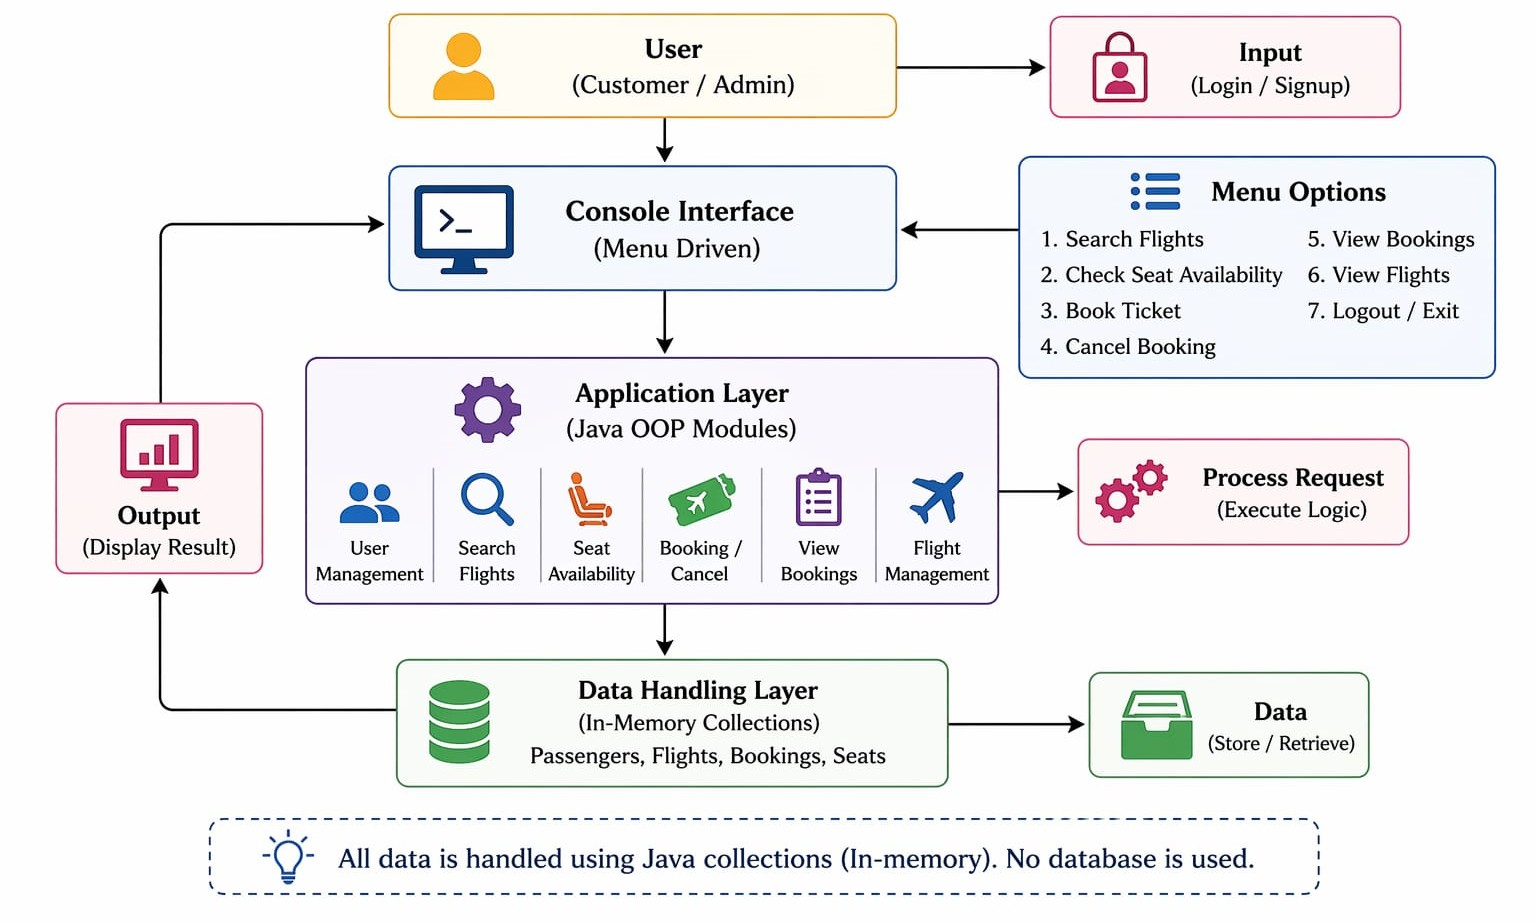
\includegraphics[width=0.9\textwidth]{ACSE_Project_Template_Field_Projects (1)/Figures/syss.jpeg}
\caption{System Architecture of Airline Reservation System}
\end{figure}

\section{Description of Architecture}

The system is designed using a three-layer architecture to ensure modularity and efficient data management.

The \textbf{Presentation Layer} is responsible for user interaction. It provides a console-based or graphical user interface through which users can search flights, book tickets, and manage reservations.

The \textbf{Application Layer} contains the core logic of the system. It is implemented using Java and includes classes such as Passenger, Flight, Booking, and Admin. This layer processes user requests and performs operations like booking, cancellation, and data validation.

The \textbf{Database Layer} stores all system data including user details, flight information, and booking records. MySQL is used as the database, and JDBC is used to connect the application with the database.

\section{System Workflow Diagram}

The workflow of the system describes the sequence of operations performed during the reservation process.

\begin{enumerate}
\item User registers or logs into the system.
\item User searches for flights by entering source and destination.
\item System displays available flights.
\item User selects a flight and proceeds to booking.
\item System checks seat availability.
\item If seats are available, booking is confirmed.
\item System updates database and displays confirmation.
\item User can cancel booking if required.
\end{enumerate}

\section{System Workflow Description}

The workflow begins when a user logs into the system. The user searches for flights based on travel details. The system retrieves available flights from the database and displays them to the user. After selecting a flight, the system checks seat availability. If seats are available, booking details are stored in the database, and confirmation is provided to the user.

If the user chooses to cancel a booking, the system updates the database and increases seat availability accordingly.

\section{Database Design}

The database is designed to manage all system data efficiently. It consists of multiple tables that store user, flight, and booking information.

\begin{itemize}
\item \textbf{Users Table:} Stores user details such as user ID, name, email, and password.
\item \textbf{Flights Table:} Contains flight information including flight ID, source, destination, timing, and available seats.
\item \textbf{Bookings Table:} Stores booking details such as booking ID, user ID, flight ID, and status.
\end{itemize}

\section{Summary}

This chapter presented the system architecture of the Airline Reservation System. It explained the layered architecture, workflow of the system, and database design. The architecture ensures efficient communication between different components and supports scalability and maintainability.